\subsection{Neural Network Design and Training}
\label{subsec:nntraining}

\begin{wrapfigure}{r}{0.5\textwidth}
	\centering
    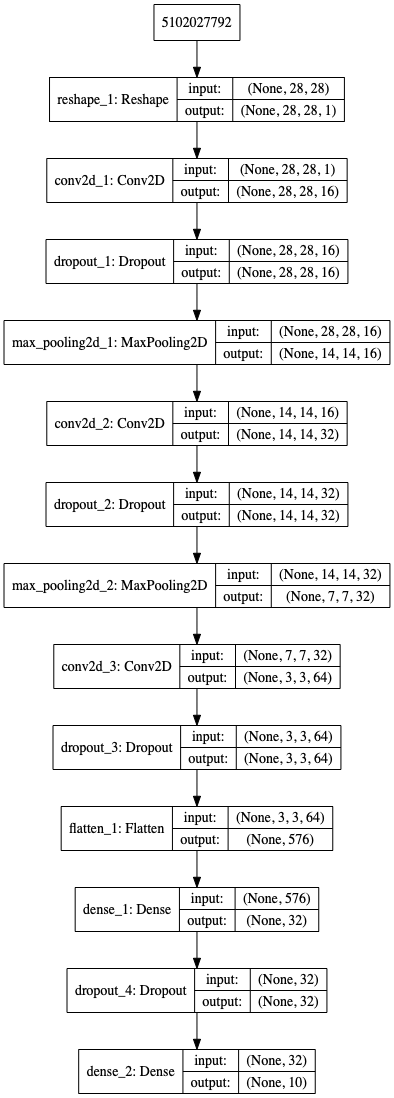
\includegraphics[width=0.35\textwidth]{img/nnlayout}
	\caption{Network Layers}
	\label{fig:network-layers}
\end{wrapfigure}

The network was implemented in PyTorch \cite{Paszke:2019aa} as well as Tensorflow \cite{MartinAbadi:2015aa}. The backend was later exclusively switched to PyTorch (which is also the most common deep learning framework in Science) due to its better support of qunatization. The layers of the network can be seen in Figure~\ref{fig:network-layers}. 
For training of the network the \emph{ADAM} optimization algorithm \cite{Kingma:2014aa} was used to minimize the cross-entropy-loss function which is defined as
\begin{equation}
    J = - y  \log(h) + (1-y)  \log(1-h)
\end{equation}
For controlling the ADAM algorithm the recommended values, listed in Table~\ref{tab:train-params}, by \cite{Kingma:2014aa} was used.
\begin{table}[ht]
	\centering
    \caption{Network Training Parameters}
    \begin{tabular}{cc}
        \toprule
            Parameter & Value \\
        \midrule
            $\alpha$   & $0.001$ \\
            $\beta_1$  & $0.9$   \\
            $\beta_2$  & $0.999$  \\          
        \bottomrule
    \end{tabular}
    \label{tab:train-params}
\end{table}
\todo{Force table to be centred in text}
\todo{Add quantization details}

A useful guide for implementing convolutions can be found in \cite{dumoulin2016guide}


\subsection{Quantization}

The network was reduced to fixed point integers defined by the equation
\begin{equation}
	v = Q \cdot 2 ^{-m}
\end{equation}
where both $Q$ and $m$ are integers and $v$ is the real value representation of the fixed point number. 

\todo{Add Histogram}
